% LaTeX-Vorlage zur Erstellung von Abschlussarbeiten an der FH Aachen
% Author: Sven Hinz
% Aenderung für FB 5: Ingo Elsen
\documentclass[11pt, a4paper, headinclude, footinclude=true, oneside]{scrreprt}
% Paket für Umlaute:
\usepackage[utf8]{inputenc}       % Cross Platform
%\usepackage[ansinew]{inputenc}   % Windows
%\usepackage[latin1]{inputenc}    % Linux
%\usepackage[applemac]{inputenc}  % Mac

\usepackage[USenglish]{babel}       % Sprache: US English
\usepackage[utf8]{inputenc} % For degree symbol in tex source
\usepackage{amsmath}
\usepackage{amsfonts}
\usepackage{amssymb}
\usepackage{makeidx}
\usepackage{graphicx}
\usepackage{epstopdf}
%\usepackage{kpfonts}
%\usepackage{textcomp}
\usepackage[left=3cm,right=3cm,top=2.5cm,bottom=2.5cm]{geometry}
%\usepackage[plainheadsepline,headsepline]{scrpage2}
\usepackage{color}
\usepackage{setspace}
%\usepackage[numbers,square]{natbib} % only required for unsrtd bib style
\usepackage{longtable}
\usepackage{listings}
\usepackage{rotating}
\usepackage{pdfpages}
\usepackage{caption}
\usepackage{subcaption}
\parindent 0pt
\usepackage{booktabs}
\usepackage[export]{adjustbox}
\usepackage{scrlayer-scrpage}
\usepackage{float} % for right positioning of pictures


% Schriftart
\usepackage{courier}
\usepackage{helvet}
\usepackage{times}
%\renewcommand{\familydefault}{\sfdefault}
%\renewcommand{\familydefault}{\rmdefault}
%\setkomafont{chapter}{\sffamily \large}
%\setkomafont{section}{\sffamily \normalsize}
%\setkomafont{subsection}{\sffamily \normalsize}
%\setkomafont{subsubsection}{\sffamily \normalsize}
%\addtokomafont{caption}{\sffamily \small}


% Abstand zwischen Kopfzeile und Kapitelüberschrift
%\renewcommand*{\chapterheadstartvskip}{\vspace*{-0.75\baselineskip}}

% Einstellungen der Kopf- und Fußzeile
\pagestyle{scrheadings}
%\ihead[\sffamily \bfseries \upshape \headmark]{\sffamily \bfseries \upshape \headmark}
\ohead[\sffamily \bfseries \upshape \headmark]{\sffamily \bfseries \upshape \headmark}
\chead[]{}
\ohead[]{}
\ifoot[]{}
\cfoot[]{}
\ofoot[\sffamily \pagemark]{\sffamily \pagemark}
\automark[]{chapter}
\renewcommand*{\chapterheadendvskip}{\vspace*{1\baselineskip}}

% Formeln
%\usepackage{fleqn} % linksbündig
%\setlength{\mathindent}{1.5cm} % Einrücktiefe

% Tabellen
\usepackage{multirow} % mehrzeiliger Text in einer Spalte
\renewcommand{\arraystretch}{2} % Zeilenabstand vergrößern
\setlength{\doublerulesep}{0.1mm} % Abstand der Doppellinien verkleinern
\usepackage{tabu}
\newcolumntype{C}{>{\centering\arraybackslash$}p{3cm}<{$}}

% Quellcode / Kommandozeileneingabe
%\lstdefinestyle{BashInputStyle}{
%language=bash,
%  basicstyle=\small\ttfamily,
  %numbers=left,
  %numberstyle=\tiny,
  %numbersep=3pt,
%  frame=tb,
%  columns=fullflexible,
  %backgroundcolor=\color{yellow!20},
%  linewidth=0.9\linewidth,
%  xleftmargin=0.1\linewidth
%}

% Inhalt
\renewcaptionname{USenglish}{\contentsname}{Contents} % Umbenennung in Inhalt

% Quellenverzeichnis
\renewcaptionname{USenglish}{\bibname}{Bibliography} % Umbenennung in Quellenverzeichnis

%\usepackage[
%  tocindentmanual,
%  tocflat,
%  tocbreaksstrict,
%  toctextentriesleft,
%]{tocstyle}

% Abkürzungsverzeichnis
%\usepackage[intoc]{nomencl}
%\let\abbrev\nomenclature
%\renewcommand{\nomname}{Abkürzungsverzeichnis}
%\setlength{\nomlabelwidth}{.25\hsize}
%\renewcommand{\nomlabel}[1]{#1 \dotfill}
%\setlength{\nomitemsep}{-\parsep}
%\makenomenclature

\usepackage[]{acronym}


\author{Nicolas Harrje} % --> Eigenen Namen einfügen


\begin{document}
\setstretch{1.1}
\addtocontents{toc}{\linespread{1}}

% Einbinden der Textinhalte mit '\include{...}'
% Die Dateien mit den Textinhalten befinden sich im Ordner 'doc'

\begin{titlepage}
	%ab hier kleinere Raender, mehr bedruckbare Flaeche.
	%\fontfamily{\sffamily}\selectfont
	\thispagestyle{empty}
	\newgeometry{a4paper, portrait, left=0cm, right=0cm, top=0.6cm, bottom=0cm, includefoot}

	% FH Logo
	\begin{flushright}
		
\includegraphics[width=1.7cm]{./pic/FHAC.jpg}
	\end{flushright}

	\vspace{-2.5cm}

	% Kopfzeile mit Fachbereich ...
	\centering \sffamily \bfseries \Large FH~Aachen \\
	\vspace{0.5cm}
	\normalsize Faculty\\
	Electrical engineering and information technology

	\vspace{1cm}

	%\centering \bfseries Bachelorarbeit
	\centering \bfseries Bachelor Thesis

	\vspace{0.8cm}

	%Titel der Arbeit
	\centering \begin{minipage}[t]{17cm}
		\centering \bfseries \large Design and Implementation of  a Performance Measurement System\\ for an Industrial Sewing Machine
		\medskip
	\end{minipage}

	\vspace{1.5cm}

	%Name und Matrikelnummer
	%\vspace*{1cm}
	%\hspace*{6.8cm}
	\begin{minipage}[t]{9cm}
		\centering Nicolas Harrje \\ Matr.-Nr.: 3518047
	\end{minipage}

	\vspace{2.1cm}

	%Professor und Betreuer
	%\vspace*{4.7cm}
	%\hspace*{6.8cm}
	\centering \begin{minipage}[t]{9cm}
		\centering \begin{tabular}{ll}
			Referent: & Prof. Dr-Ing. ...\\
			Korreferent: & Prof. Dr.-Ing. ...\\
			%Externer Betreuer: & Dipl.-Wirt.-Ing\\
		\end{tabular}
	\end{minipage}

	\vspace{7cm}

	% Firmenlogo
	%\begin{flushleft}
	%\centering \hspace{-8cm}
	%\begin{minipage}[t]{5cm}
			%\includegraphics[width=5cm]{./pic/firmenlogo.jpg}
	%\end{minipage}
	%\end{flushleft}


	%Erstellungsdatum
	%\vspace{-4cm}
	%\begin{flushright}
	\centering %\hspace{8cm}
	\begin{minipage}[b]{5cm}
			\centering
			\today\\ %Datum\\
			%\vspace{1cm}
			%In Zusammenarbeit mit\\
			%Firma, Ort\\
			%\vspace{1cm}
			%vertraulich bis xx.xx.xx
	\end{minipage}
	%\end{flushright}

	%\today
	\restoregeometry
\end{titlepage}


\clearpage
\chapter*{Erklärung}\label{erklaerung}
\markboth{Erklärung}{Erklärung}
Ich versichere hiermit, dass ich die vorliegende Arbeit selbstständig verfasst und keine anderen als die im Literaturverzeichnis angegebenen Quellen benutzt habe.

\bigskip

Stellen, die wörtlich oder sinngemäß aus veröffentlichten oder noch nicht veröffentlichten Quellen entnommen sind, sind als solche kenntlich gemacht.

\bigskip

Die Zeichnungen oder Abbildungen in dieser Arbeit sind von mir selbst erstellt worden oder mit einem entsprechenden Quellennachweis versehen.

\bigskip

Diese Arbeit ist in gleicher oder ähnlicher Form noch bei keiner anderen Prüfungsbehörde eingereicht worden.

\vspace{1cm}
Aachen, \today %Monat Jahr

\vspace{7cm}
\section*{Geheimhaltung - Sperrvermerk}\label{geheimhaltung}

Die vorliegende Arbeit unterliegt bis [Datum] der Geheimhaltung. Sie darf vorher weder vollständig noch auszugsweise ohne schriftliche Zustimmung des Autors, des betreuenden Referenten bzw. der Firma [Firmenname und -sitz] vervielfältigt, veröffentlicht oder Dritten zugänglich gemacht werden.

%\clearpage
\chapter*{Danksagung}\label{danksagung}
\markboth{Danksagung}{Danksagung}
Danke.

% Inhaltsverzeichnis
\clearpage
\makeatletter
\renewcommand*{\@dotsep}{1} % Punktabstand einstellen
\makeatother
\tableofcontents

% Das erste Kapitel soll auf einer ungeraden Seite beginnen.
\cleardoublepage
\setstretch{1.1}

% Nicht benötigte Kapitel können auskommentiert werden
% Für zusätzliche Kapitel müssen weitere Dateien im Ordner 'doc' angelegt werden

\clearpage
\chapter{\textbf{Introduction}}\label{introduction}
Industrial sewing machines are of crucial importance in the textile industry, where they are typically utilized in the final stage of production to assemble the end product. This stage necessitates the highest level of human involvement, thereby becoming a pivotal element in determining both production efficiency and product quality. Therefore, the implementation of performance measurement techniques is particularly appropriate in this context. In the field of performance measurement, the seminal work by Neely \cite{neelyPerformanceMeasurementSystem1995} is widely cited. They defined performance measurement as "[...] the process of quantifying the efficiency and effectiveness of action." . This is frequently achieved through the implementation of Key Performance Indicators (KPIs), as they are formally standardized in the ISO 22400 framework, which governs operations management and production.
\\\\
In recent years, the popularity of automatic systems for performance measurement on sewing machines has increased. Nonetheless, these systems continue to encounter certain challenges that have frequently been overlooked. Firstly, it must be acknowledged that a considerable number of systems are dependent on cloud technology. This reliance engenders certain issues, including elevated latency and the perpetual financial obligations associated with cloud usage. Secondly, the utilization of standards and frameworks is frequently neglected, which results in the complexity of scaling and maintaining these systems. Thirdly, the prevailing focus of numerous works in this field is retrofitting sewing machines, rather than utilizing the machine's inherent data, which often leads to the production of erroneous results. Fourthly, the dearth of software architecture that utilizes services engenders considerable challenges in achieving scalability.
\\\\
The objective of this thesis is to establish a replicable methodology for designing and implementing a performance measurement system, with a sewing machine serving as a case study. This encompasses the provision of an overview of standards frameworks and technologies, in addition to the demonstration of the selection process for the most suitable option and its subsequent implementation. This thesis proposes a system that maximizes the use of actively maintained open-source technologies while ensuring easy scalability for future expansion. The end result will be a dashboard that provides the most important KPIs (such as cycle time, OEE, setup time, and down time) in real time.
\\\\
The scope of this work is limited to a Brother sewing machine of type UF-8910, which is connected to a WAGO PLC of type 750-8101 PFC100 CS 2ETH. The WAGO PLC employs the OPC-UA protocol for data transmission to the network. The anticipated data flow and signals are modeled and do not originate from the physical sewing machine and PLC. The sewing machine is part of a shop-floor that is used for workshops where industry customers can gain insight into productivity and quality enhancements within production environments through digitization. The system outlined in this thesis is intended to serve as a demonstrative model, and as such, it will feature visualizations that elucidate its real-time capabilities. The derivation of KPIs must be constrained to those that require querying from the database without necessitating additional post-processing.
\\\\
The relevance of this thesis is predicated on the increasing demand for data-driven decision-making to optimize efficiency and reduce costs, a phenomenon that is especially pronounced in the highly competitive garment industry. Performance measurement systems empower production management to identify inefficiencies and minimize unproductive periods. Furthermore, they furnish actionable insights that facilitate targeted operator coaching. This thesis makes a significant contribution to the extant knowledge base concerning IoT-based monitoring systems, as it focuses on replicable methods. This as well as the focus on open source technology make the system architecture well suited for small and medium sized companies with limited resources.
\\\\
This thesis employs a design-science approach, with the sewing machine performance measurement system serving as the artifact. A literature review is also employed to provide a comprehensive overview of the extant related work, as well as the frameworks, standards, and technologies relevant to the subject. To further implement suitable technology solutions, a structured technology selection process is being developed and followed.
\\\\
In the following, the structure of this thesis is being outlined. The initial section presents the foundational technologies, frameworks, standards, and other groundwork upon which this work is based. The related work section then reviews relevant literature, examining systems with similar objectives to contextualize and position the approach proposed in this thesis. Subsequently, the requirements and system design section details the specific needs addressed by the system, as well as the selected KPIs and technologies. Building on this foundation, the implementation of the system is described. The subsequent evaluation section provides an analysis of the system’s strengths and limitations. Finally, the outlook and conclusion offer a summary of the findings and discuss potential directions for future development.


 % Einleitung
\clearpage
\chapter{\textbf{Foundations}}\label{grundlagen}
%\addtocontents{toc}{\vspace{0.8cm}}
\section{Setting}
The sewing machine in question is a Brother UF-8910.It is part of a textile production line in which a wristband is being produced. The wristband contains an RFID chip capable of storing diverse information. For instance, the technology could be utilized to store a personnel identification number. In the event that the technology is scanned at a workplace, the workplace's dimensions would adapt to conform to the worker's size. The production line has not been designed for implementation in actual industrial-scale manufacturing; rather, it functions as a model environment for workshop purposes. The sewing machine is utilized during the final stage of the wristband assembly process. The utilization of the machine is characterized by a straightforward procedural nature. The objective is to sew both ends of the open wristband together with a single seam to close it. The following figure illustrates this procedure.\\
\textbf{figure}
\\

The signals that can be extracted from the sewing machine encompass:
\begin{itemize}
	\item Second walking foot stroke: Two walking foot strokes can be set for different thikness of materials. This signal indicates if the walking foot is currently in the second stroke hight.
	\item Thread trimming: Indicates when the thread is trimmed
	\item Pressure foot: Indicates if the pressure foot is lifted
	\item Upper shaft rotating: Indicates if the machine is actively sewing
	\item Other than home screen: Indicates that the menu screen is currently not in the home screen
	\item Home screen and not sewing: Indicates that the menu screen is in the home screen and the machine is not actively sewing
\end{itemize}
The subsequent figure illustrates the various components of the sewing machine, thereby facilitating a more profound comprehension of the signals.\\
\textbf{figure}
\section{Definitions}
\subsection{Takt Time}
Maximum time allowed to produce one product in order to meet customer demand
\subsection{IoT and IIoT}
The term Internet of Things was first coined by \cite{ashtonThatInternetThings} when explaining the idea of combining RFID with the internet in an executive meeting. He explains that on the "normal" internet, most of the content is created by human beings. In contrast to this in the Internet of Things the data is generated by things and often describes things. But his emphasizes lays more on the description of things. For example to track and count them. The information to do so would come from sensors and RFID, he says.
Of course in these days more of the information on the internet is generated by bots and AI. But other than that the distinction still holds true. 
\\The Internet Society \cite{roseInternetThingsOverview} further explains that in the Internet of Things, machines are communicating with each other and are addressable via an own IP address. This standardizes the way in which devices communicate. They also mention that "Today, the Internet of Things has become a popular term for describing scenarios in which  Internet connectivity and computing capability extend to a variety of objects, devices, sensors, and everyday  items."
\\The Industrial Internet of Things is just the description of a domain where the IoT is used. In this case in manufacturing. \cite{WhatIoTInternet}
\section{State of the Art}\label{unterkapitel}
\subsection{Industrial IoT Architectures and Patterns}
Due to the requirement that the solution be developed utilizing IoT technologies and is set within a production context, a review of Industrial IoT (IIoT) architectures and patterns was conducted. The Industrial Internet Reference Architecture (IIRA) \cite{youngIndustrialInternetReference2022} serves as a comprehensive framework, offering valuable insights into various architectural models and design patterns relevant to this domain. This reference architecture describes the following patterns: IoT Component Capability Pattern, Three-Tier Architecture Pattern, Gateway-Mediated Edge Connectivity and Management architecture pattern, Digital Twin Core as a Middleware Architecture Pattern, Layered Databus Architecture Pattern, System-of-Systems Orchestrator Architecture Pattern. Of these patterns only the first two are applicable within the scope of this work. Therefore the other ones will only be described on the surface.
\paragraph{Architecture Patterns}
IoT architecture patterns define the structure and operation of various IoT systems, detailing their implementation and highlighting their unique characteristics.
\subparagraph{IoT Component Capability Model Pattern}
A single component and its associated capabilities are described, with the possibility that a component may comprise multiple sub-components. Consequently, the entire system can also be regarded as a component. The specific meanings of the capabilities are illustrated in the accompanying figure.
\begin{figure}[H]
	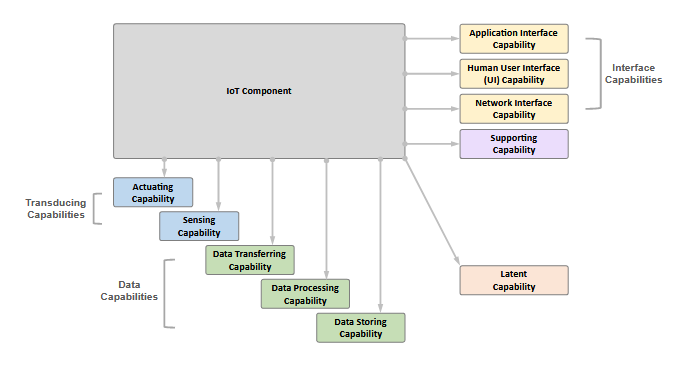
\includegraphics[width=\linewidth]{pic/IIRA-model-component-pattern.png}
	\caption{Component Capability Pattern. \\ (Young et al., 2022, S. 40)}
	\label{fig:Model-Component-Pattern}
\end{figure}
\subparagraph{Three-Tier Architecture Pattern}
The system comprises the Edge, Platform, and Enterprise Tiers, as well as connecting networks. The Edge Tier contains sensors and gateways that collect data. These are connected by the Proximity Network. Data preprocessing may already be happening there.
\\The Platform Tier is responsible for most data processing and storage via databases. It is connected to the Edge Tier via the Access Network.
\\The Enterprise Tier provides domain-specific applications and interfaces for end users. These are built upon the processed data from the platform tier. It also issues controls to lower tiers. This tier is connected to the Access Network via the Service Network.
The three tiers can also be further divided into different domains. That makes sense for bigger systems. But for a simple system as the one described in this work it is not necessary and therefore these domains will not be explained here.
\begin{figure}[H]
	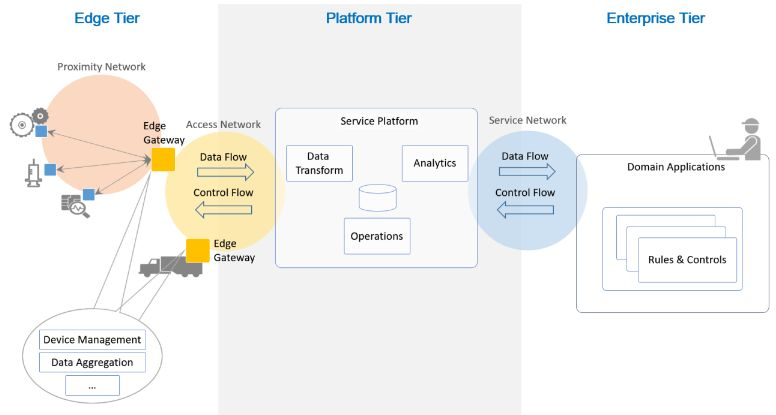
\includegraphics[width=\linewidth]{pic/three-tier-architecture.jpg}
	\caption{Three Tier Architecture \\ (Young et al., 2022, S. 44)}
	\label{fig:Three-Tier-Architecture}
\end{figure}
\subsection{KPIs and Metrics for Performance Evaluation in Sewing Operations}
Performance measurement in the textile production industry is important due to intense competition. It enables producers to identify potential bottlenecks, provides a deeper understanding of processes, and facilitates more effective resource allocation \cite{alauddinProcessImprovementSewing2018}.
\\Key performance indicators (KPIs) and metrics serve as essential tools for performance measurement. Kang et al. \cite{kangHierarchicalStructureKey2016} from the National Institute of Standards and Technology in the United States analyzed the relationships among various types of KPIs and metrics used in operations management and production, based on the ISO 22400 standard.
Supporting elements, referred to as metrics in this thesis, describe the measured data necessary for calculating basic KPIs. These supporting elements are categorized into time and quantity.
Time elements quantify the duration of various events, such as the production time per unit. Conversely, quantity elements pertain to the number of produced items.
Maintenance elements capture information about machine-related issues. 
\\Based on the supporting elements, basic KPIs can be calculated. These KPIs are categorized into production, quality, and maintenance KPIs.
\\The researchers also emphasize the importance of comprehensive KPIs, which provide a broader overview of production performance. These KPIs build upon basic KPIs and include, for example, Overall Equipment Effectiveness (OEE), which is calculated by multiplying the KPIs for availability, performance, and quality ratio.
\\Other studies \cite{kironKPIKeyPerformance2022, alauddinProcessImprovementSewing2018} have specified KPIs specifically for the sewing section of a textile production plant. In this context, some KPIs overlap with those examined by Kang et al., while additional KPIs unique to the sewing section have also been introduced. The following table classifies these sewing-specific KPIs within the hierarchical framework proposed by Kang et al.
\begin{longtable}{|p{3cm}|p{7cm}|p{4cm}|}
	\caption{Classification of KPIs and Metrics in Sewing Section (based on Kang et al., 2016 and ISO 22400)} \\
	\hline
	\textbf{KPI/Metric} & \textbf{Description} & \textbf{Classification (Kang et al., 2016 / ISO 22400)} \\
	\hline
	\endfirsthead
	
	\hline
	\textbf{KPI/Metric} & \textbf{Description} & \textbf{Classification (Kang et al., 2016 / ISO 22400)} \\
	\hline
	\endhead
	% --- Supporting Element: Time ---
	\multicolumn{3}{|l|}{\textbf{Supporting Element: Time}} \\
	\hline
	Cycle Time & Total time taken to complete one operation, from start to start of the next piece. & Supporting Element: Time \\
	\hline
	Standard Minute Value (SMV) & Time required to complete a specific job under standard conditions and pace. & Supporting Element: Time \\
	\hline
	Allowance & Extra time permitted for personal needs, delays, and fatigue in production. & Supporting Element: Time \\
	\hline
	Idle Time/Machine & Time when operators or machines are not working, considered lost time. & Supporting Element: Time \\
	\hline
	% --- Supporting Element: Quantity ---
	\multicolumn{3}{|l|}{\textbf{Supporting Element: Quantity}} \\
	\hline
	Operation & A step in the process required to convert materials into a finished product. & Supporting Element: Quantity \\
	\hline
	Manpower to Machine Ratio & Ratio of workers to machines, used to optimize labor and production. & Supporting Element: Quantity \\
	\hline
	Absenteeism & Rate of operator absence, which affects production and efficiency. & Supporting Element: Quantity \\
	\hline
	No of Style Change & Frequency of style changes, impacting productivity, efficiency, and quality. & Supporting Element: Quantity \\
	\hline
	% --- Basic KPI: Production ---
	\multicolumn{3}{|l|}{\textbf{Basic KPI: Production}} \\
	\hline
	Efficiency & Comparison of actual output to what could be achieved with the same resources. & Basic KPI: Production \\
	\hline
	Productivity & Achievement toward goals based on the relationship between inputs and outputs. & Basic KPI: Production \\
	\hline
	Availability & Percentage of scheduled time employees or machines are productive. & Basic KPI: Production \\
	\hline
	Performance & Amount of product delivered relative to available productive time. & Basic KPI: Production \\
	\hline
	Line Wise Sewing Efficiency & Efficiency of sewing lines, often linked to man-to-machine ratio. & Basic KPI: Production \\
	\hline
	% --- Basic KPI: Quality ---
	\multicolumn{3}{|l|}{\textbf{Basic KPI: Quality}} \\
	\hline
	Defect per Hundred Units (DHU) & Number of defects found per hundred units produced. & Basic KPI: Quality \\
	\hline
	Quality & Percentage of perfect or saleable products produced. & Basic KPI: Quality \\
	\hline
	% --- Comprehensive KPI ---
	\multicolumn{3}{|l|}{\textbf{Comprehensive KPI}} \\
	\hline
	Overall Labor Effectiveness (OLE) & Measures workforce utilization, performance, and quality, reflecting labor's impact on productivity. & Comprehensive KPI \\
	\hline
	Overall Equipment Effectiveness (OEE) & Quantifies how well equipment performs relative to its designed capacity, considering availability, performance, and quality. & Comprehensive KPI \\
	\hline
\end{longtable}
\subsection{IoT-Plattforms}
The IoT is known for producing large amounts of data and for the potentials to grow these amounts even more. Therefore a scalable software infrastructure that is needed. That is where IoT-Plattforms come into play \cite{turkiEvaluatingOpenSource2024}. The authors also mention that IoT-Platforms help accelerating the solution development "[...] by providing foundational capabilities, avoiding the need to implement low-level infrastructure."
\\\cite{asemaniUnderstandingIoTPlatforms2019} further highlight the different capabilities that are typical for IoT-Platforms.
\paragraph{Connectivity and Device Management}
Through various communication protocols the platforms connect with the devices, enabling them to communicate with each other, manage device status and configurations, handle software updates and provide mechanisms for error reporting.
\paragraph{Data Storage, Management, Analysis, Visualization}
Through connections to databases they store large volumes of data often in the cloud or locally. Also further data processing and analytics through various methods as well as visualizations through dashboards are possible.
\paragraph{Development and Deployment Tools}
By providing APIs and SDKs the developers are enabled to further create custom applications.
\paragraph{Auditing and Payments}
The Platforms help to have an overview over the data or compute usage and the resulting costs.
\paragraph{Service Management}
By giving an oversight over parameters like resource consumption, data requirements and access, the user can monitor vertical as well as platform internal services. The platforms also enable the communication between services or combination of basic services to create new ones.
\paragraph{Integration}
Platforms can be integrated with each other, other data sources and the cloud. 
\paragraph{Fog/Edge Computing}
IoT-Platforms often support distributed data processing and storage. This can lead to less traffic due to processing close to the data source. Faster transmission would be enabled therefore and reinforced due to  shorter communication distances.
\\\\The researchers go on to reveal that while commercial platforms carry all of the mentioned capabilities, open source platforms are often focused on specific capabilities. Thus in implementation sometimes need to be combined to deliver a holistic IoT-Platform. 
\subsection{Differences between Relational and Timeseries Databases}
In the paper written by \cite{turkogluComparisonTimeSeries2024} it is analyzed how relational databases and time series databases compare regarding speed and storage efficiency when used in Grafana.
First they point out the use case for relational databases is for single time data points, which can be related to other data points over various tables. Therefore enabling complex queries involving joins, aggregations and multiple tables. They make sure the data is accurate and stays consistent.
Time series data bases on the other hand are made for data points with a timestamp and large volumes of data. This makes them ideal for IoT applications and real time data analytics. They are optimized to enable high speed read and write operations as well as efficient data storage.
The differences in query return time are already there with small amounts of data, but when scaling up the amount they become clearly visible as can be seen in the figure below.
\begin{figure}[H]
	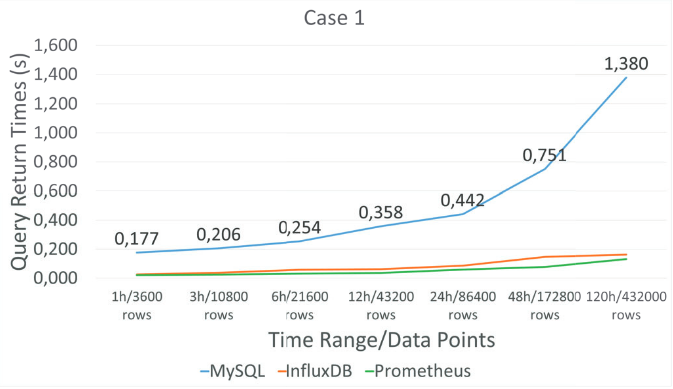
\includegraphics[width=\linewidth]{pic/query-performance-db.png}
	\caption{Query Performance Relational vs. Time Series DB \\ (Turkoglu et. al, 2024, S. 2)}
	\label{fig:query-performance-db}
\end{figure}
This is only one of three test cases but they all give a similar picture that shows the superiority of time series databases regarding query return times.

\subsection{Dashboarding}
\addtocontents{toc}{\vspace{0.8cm}}



\chapter{\textbf{Requirements Analysis}}\label{grundlagen}
In order to select the most suitable technologies and design the system, it is first necessary to establish clear requirements. In this chapter, the aforementioned requirements will be enumerated and elucidated.
In order to maintain consistency regarding the compliance level, the terms "must," "should," and "will" were employed.
The following words shall be explained in brief. The term "must" is employed to signify an unconditional obligation, implying that the fulfillment of this requirement is not subject to discussion or negotiation. The term "should" conveys a degree of desirability, indicating that fulfillment of the requirement would be advantageous. The term "will" signifies that this particular requirement is currently under consideration for inclusion in the subsequent release. However, it is imperative to maintain awareness of this requirement so that the system can be designed in a manner that facilitates its seamless integration in the future.
\subsection{Functional System Requirements} % (from your requirements table)
\begin{tabularx}{\textwidth}{|X|X|}
	\hline
\textbf{Requirement}	& \textbf{Explanation} \\
	\hline
The system must show KPIs that are relevant for the sewing process	&  In the workshops there must be some KPIs that fit into the story of a textile production with a sewing process\\
	\hline
The system should show aditional KPIs that are relevant for the manufacturing industry in general	&  Workshop participants are from all sorts of companies within the manufacturing industry\\
	\hline
 The system must present these KPIs in a visual manner that provides information about the classification of the current value e.g. with colors and thresholds	& So that the management can act quickly upon the KPIs and does not need to lookup thresholds \\
	\hline
The system must provide the user with the ability to change the timeframe on which the KPIs are calculated	&  Especially when looking at historic data it is usefull to be able to set the timeframe\\
	\hline
The system should show graphs with historical data & Enables management to see trends and patterns\\
	\hline
\end{tabularx}

\subsection{Non-Functional Requirements} %(scalability, security, real-time processing)
\begin{tabularx}{\textwidth}{|X|X|}
	\hline
\textbf{Requirement}	&  \textbf{Explanation}\\
	\hline
The system must make use of open source software where possible	&  To be replecable by small and medium companies\\
	\hline
The system must be capable to generate all of the KPIs from the machine-data without installing any additional sensors	&  \\
	\hline
The system must be designed in a way that makes it easily scalable	&  \\
	\hline
The system must be deployable with minimal effort	&  \\
	\hline
The system must be capable to retrieve raw data via opc-ua	&  \\
	\hline
The system should make use of existing patterns, frameworks and solutions were possible	&  \\
	\hline
The system should update the KPIs in real-time (<10s)	&  \\
	\hline
 The system must be able to run on a local machine and therefore independent of any cloud service	&  \\
	\hline
The system must provide the user with the ability to access the dashboard from within the shopfloor network	&  \\
	\hline
\end{tabularx}

\subsection{Constraints} %(no additional sensors, existing infrastructure)
\subsection{KPI Selection and Justification}
 Of which the following were able to be calculated with the given metrics.
\\
\clearpage
\chapter{\textbf{Zusammenfassung und Ausblick}}\label{zusammenfassung}
\addtocontents{toc}{\vspace{0.8cm}}


% Nachspann
\nocite{Segmentation} % Quelle wird nicht im Text erwähnt -> Quellenverzeichnis
\nocite{ImageAttack}
% Weitere quellen müssen in 'bib/quellen.bib' eingetragen werden
% !!! -> BibTex ausführen! Sonst tauchen die Quellen nicht im Verzeichnis auf.

% Quellenverzeichnis
\clearpage
%\bibliographystyle{alpha}
\bibliographystyle{apalike}
\bibliography{./bib/quellen}
\addcontentsline{toc}{chapter}{Quellenverzeichnis}
%\addtocontents{toc}{\vspace{0.8cm}}

% Abkürzungsverzeichnis
\clearpage
\markright{Abkürzungsverzeichnis}
\clearpage
\chapter*{Abkürzungsverzeichnis}\label{abkuerzungsverzeichnis}
\addcontentsline{toc}{chapter}{Abkürzungsverzeichnis}
\begin{acronym}[YTM]
\setlength{\itemsep}{-\parsep}

\acro{IoT}[$IoT$]{\hspace{1cm}Internet of Things}
\acro{IIoT}[$IIoT$]{\hspace{1cm}Industrial Internet of Things}
\acro{KPI}[$KPI$]{\hspace{1cm}Key Performance Indicator}
\acro{PLC}[$PLC$]{\hspace{1cm}Programmable Logic Controller}
\acro{OPC UA}[$OPC UA$]{\hspace{1cm}Open Process Control Unified Architecture}
\acro{DBMS}[$DBMS$]{\hspace{1cm}Database Management System}
\acro{TS-DBMS}[$TS-DBMS$]{\hspace{1cm}Timeseries Database Management System}
\acro{}[$x$]{\hspace{1cm}x}


\end{acronym}

%\addtocontents{toc}{\vspace{0.8cm}}

% Abbildungsverzeichnis
\clearpage
\addcontentsline{toc}{chapter}{Abbildungsverzeichnis}
\listoffigures
%\addtocontents{toc}{\vspace{0.8cm}}

% Tabellenverzeichnis
\clearpage
\addcontentsline{toc}{chapter}{Tabellenverzeichnis}
\listoftables
\addtocontents{toc}{\vspace{0.8cm}}

% Anhaenge
\addcontentsline{toc}{chapter}{Anhang}
\appendix
%\input{./app/Dateiname}
\chapter{Quellcode}
\begin{enumerate}
      \item Source 1
      \item Source 2
\end{enumerate}

% Anhänge im Ordner 'app' ablegen

%\includepdf[pages=1-4]{./app/Datenblatt1.pdf} % Datei mit 4 Seiten
%\includepdf[pages=1]{./app/Datenblatt2.pdf} % Datei mit einer Seite

\chapter{Rohdatenvisualisierungen}
\begin{enumerate}
      \item Graustufen
      \item Verteilungen
\end{enumerate}
\end{document}
